%----------------------------------------------------------------------------------------
%	PACKAGES AND THEMES
%----------------------------------------------------------------------------------------
\PassOptionsToPackage{table}{xcolor}
\documentclass[aspectratio=169,xcolor=dvipsnames,svgnames,x11names,fleqn]{beamer}
% \documentclass[aspectratio=169,xcolor=dvipsnames,fleqn]{beamer}

\usetheme{RedVelvet}

\usefonttheme[onlymath]{serif}
\newcommand{\showanswers}{yes}


\usepackage{xspace}
\usepackage{amsmath}
\usepackage{amssymb}
\usepackage{amsfonts}
\usepackage{color}
\usepackage{physics}
% \usepackage{mathbb}
\usepackage{rahul_math}
\usepackage{bigints}

\usepackage{graphicx} % Allows including images
\usepackage{booktabs} % Allows the use of \toprule, \midrule and \bottomrule in tables
\usepackage{tikz,pgfplots}

\usepackage{subfigure}
\usetikzlibrary{arrows}
\usepackage{minted}
\definecolor{LightGray}{gray}{0.9}
\definecolor{cream}{rgb}{0.92, 0.9, 0.55}
\definecolor{lightblue}{rgb}{0.68, 0.85, 0.9}


\usepackage{xcolor-material}
\usetikzlibrary{fit}
\usetikzlibrary{matrix}
\tikzset{%
apple/.pic={
  \fill [MaterialBrown] (-1/8,0)  arc (180:120:1 and 3/2) coordinate [pos=3/5] (@)-- ++(1/6,-1/7)  arc (120:180:5/4 and 3/2) -- cycle;
  \fill [MaterialLightGreen500] (0,-9/10)  .. controls ++(180:1/8) and ++(  0:1/4) .. (-1/3,  -1) .. controls ++(180:1/3) and ++(270:1/2) .. (  -1,   0) .. controls ++( 90:1/3) and ++(180:1/3) .. (-1/2, 3/4) .. controls ++(  0:1/8) and ++(135:1/8) .. (   0, 4/7)
}
}

\newcommand{\leftdoublequote}{\textcolor{blue}{\scalebox{3}{``}}}

\newcommand{\rightdoublequote}{\textcolor{blue}{\scalebox{3}{''}}}


\usepackage{textcomp}

\usepackage{overpic}

%----------------------------------------------------------------------------------------
%	TITLE PAGE
%----------------------------------------------------------------------------------------

\usepackage{tikz-qtree,tikz-qtree-compat}
\usetikzlibrary{calc}


\title[CPE 486/586: Machine Learning]{CPE 486/586: Machine Learning for Engineers} % The short title appears at the bottom of every slide, the full title is only on the title page
\subtitle{04Bonus Data Visualization}

\author[Rahul Bhadani] {{\Large \textbf{Rahul Bhadani}}}

\institute[UAH] % Your institution as it will appear on the bottom of every slide, maybe shorthand to save space
{
    Electrical \& Computer Engineering,  The University of Alabama in Huntsville
}
\date

% \titlegraphic{
%    \includegraphics[width=0.4\linewidth]{figures/UAH_primary.png}
% }

\begin{document}

%-------------------------------------------------
\begin{frame}
    \titlepage
\end{frame}

%-------------------------------------------------
\begin{frame}{Outline}
    \backgroundtableofcontents
\end{frame}


%------------------------------------------------
\section{Data Exploration}
%------------------------------------------------

%------------------------------------------------
\begin{frame}{}
\begin{center}
    \huge \bf \color{DarkRed}
    Data Exploration
\end{center}
\end{frame}

\begin{frame}{Why Data Exploration?}
    \begin{facts}{}
        \begin{enumerate}
            \item Data exploration is useful to answer a number of questions about data, thereby corroborating or invalidating hunches and preconceptions.
            \item Data exploration reveals unexpected patterns, trends, and exceptions as well as stimulates new perspectives and insights.
        \end{enumerate}
    \end{facts}
\end{frame}

\begin{frame}{Understanding Different Types of Data and Data Structure}
    \begin{gradbox}{}
        \begin{enumerate}
            \item What type of data is right for the question you are answering?
                \begin{enumerate}
                    \item In-class exercise: Consider a question you are interested in. What type of data would you be collecting?  
                \end{enumerate}
            \item Extract, use, and organize your data.
            \item Make sure the data is relevant and valid.
            \item Learn how data is generated \& collected.
            \item Different formats, types, and structures of data.
            \item What does clean data mean?
        \end{enumerate}
    \end{gradbox}
\end{frame}

%------------------------------------------------

\begin{frame}{Ubiquity of Data in the Modern World}
Data is generated all around the world in the form of texts, pictures, videos, emails, through social media, mobile phones, etc.

    \begin{columns}[c] % The "c" option specifies centered vertical alignment while the "t" option is used for top vertical alignment

        \column{.15\textwidth} % Left column and width
        
\includegraphics[width=0.8\textwidth]{figures/document.png}

        \column{.15\textwidth} % Right column and width
        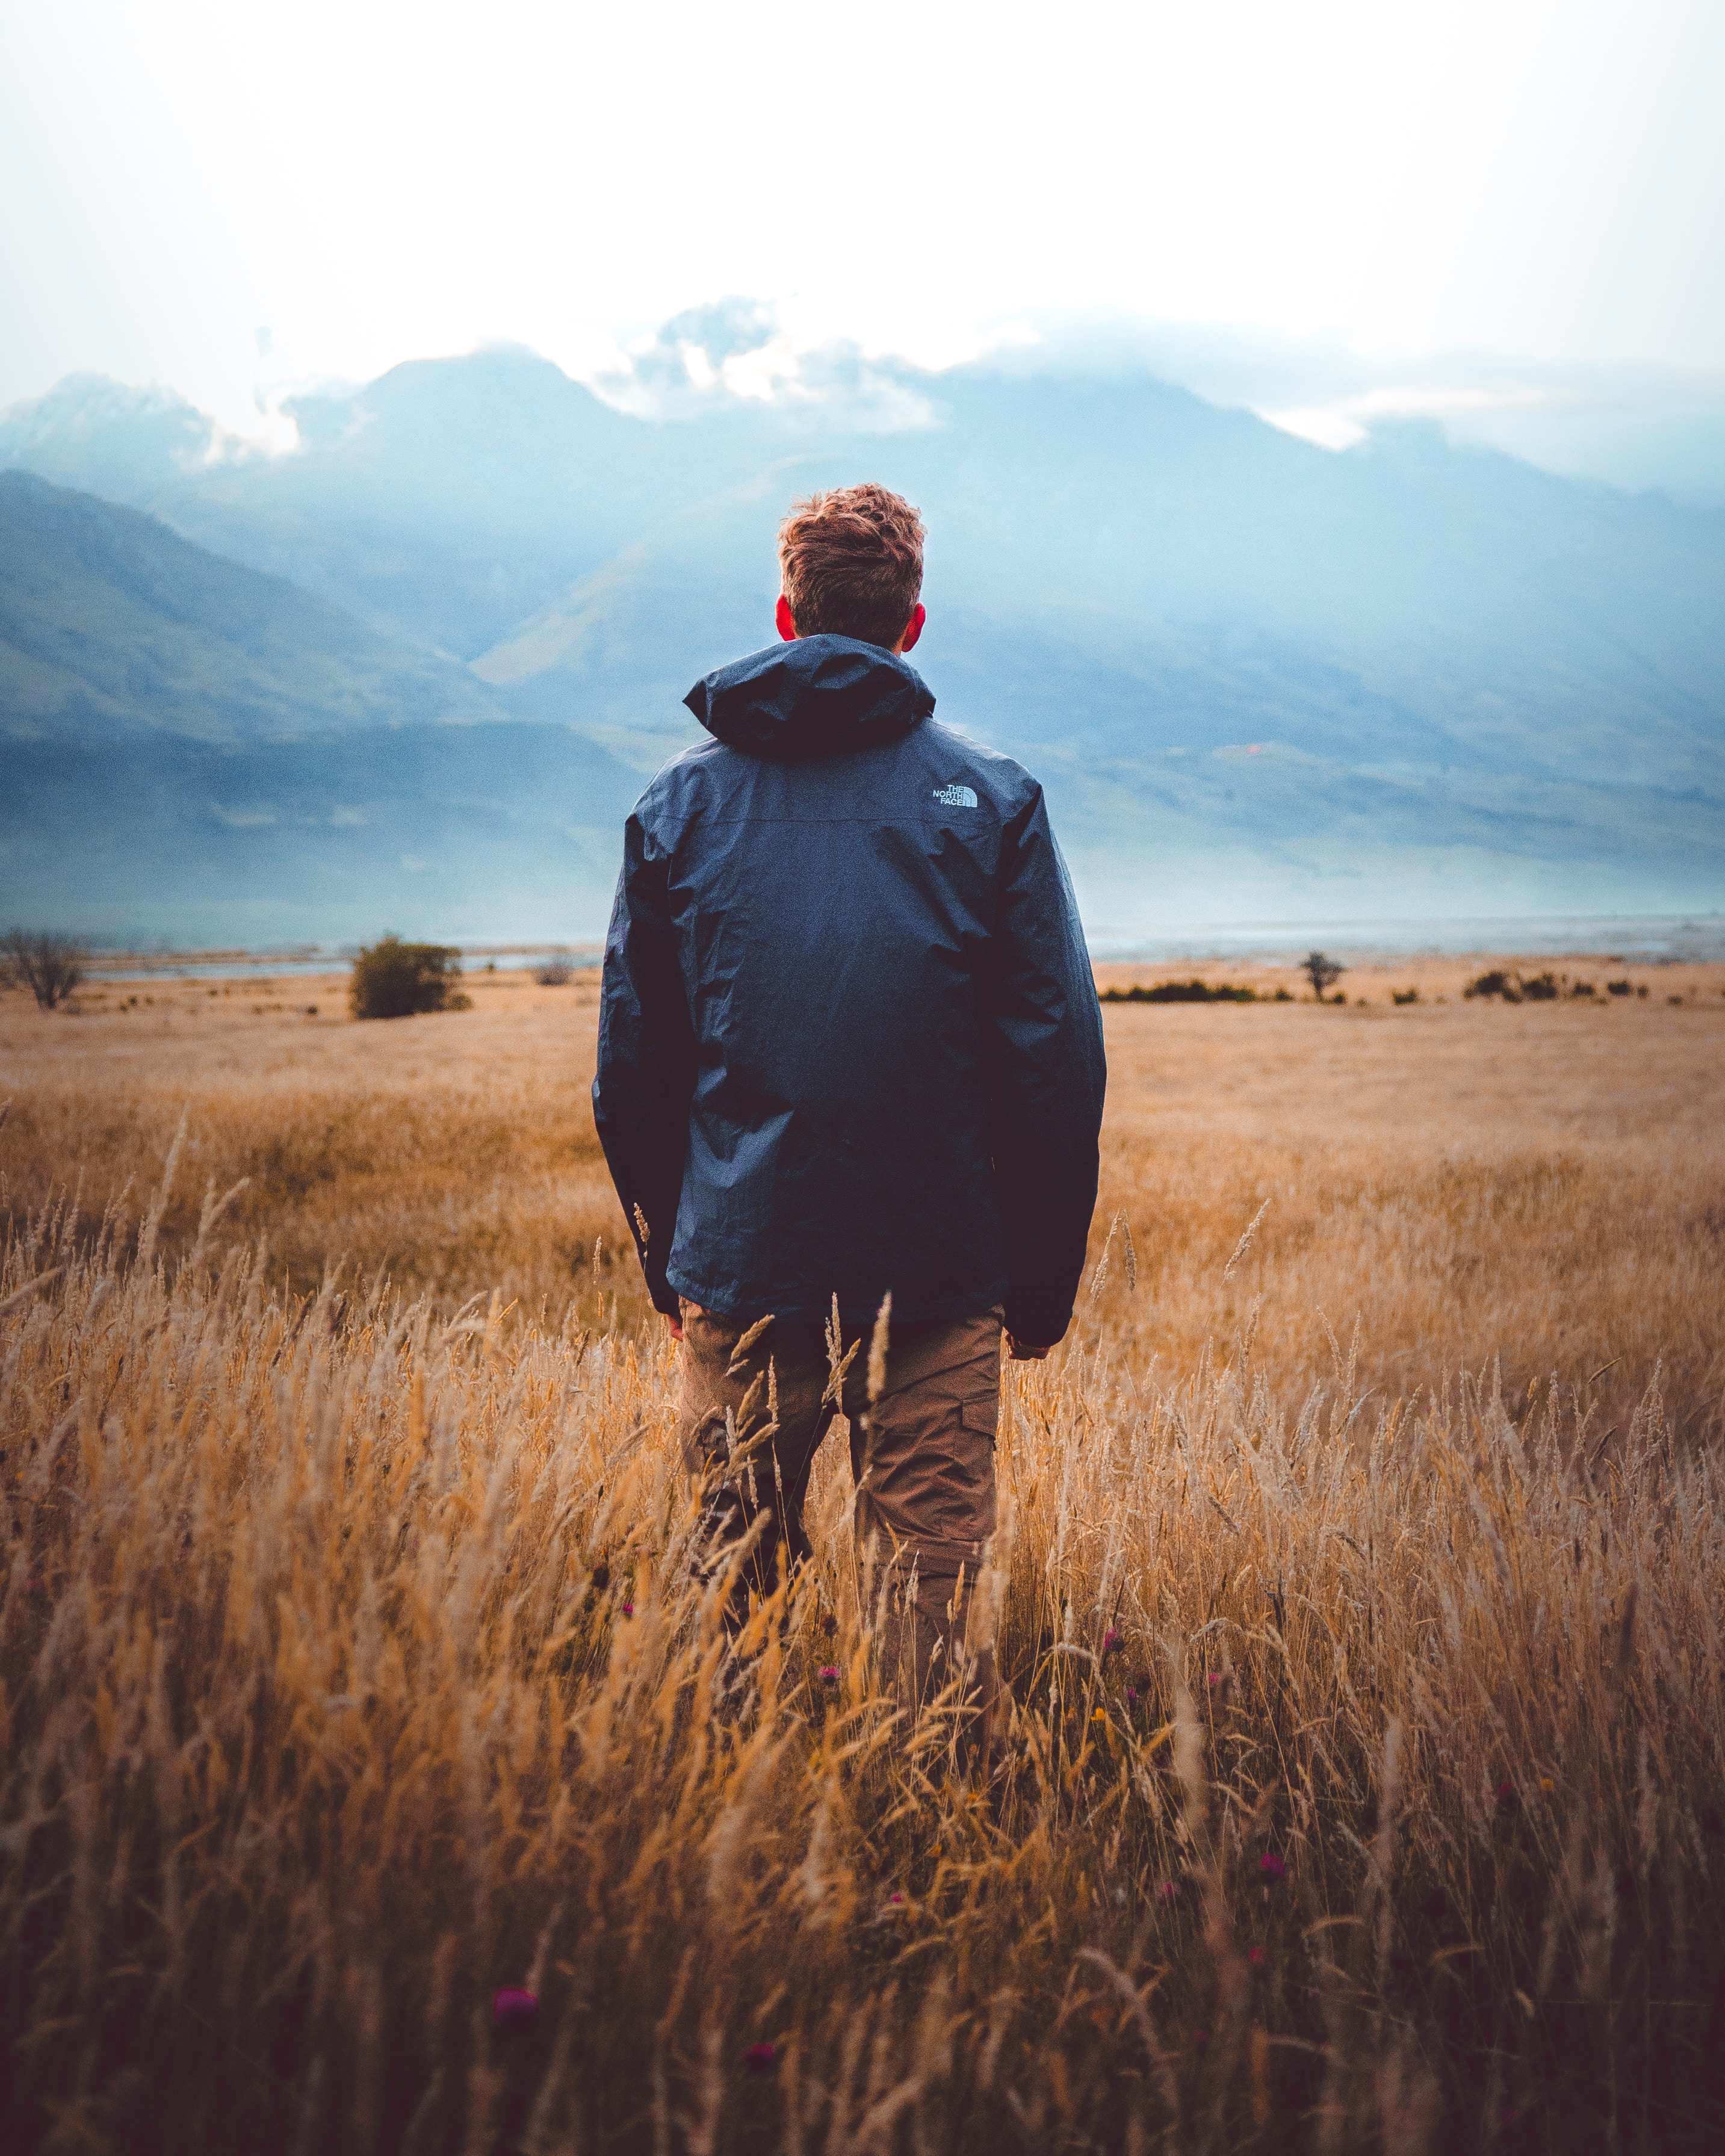
\includegraphics[width=.8\textwidth]{figures/image.jpg}

        \column{.15\textwidth} % Right column and width
        
\includegraphics[width=.99\textwidth]{figures/video.png}

        \column{.15\textwidth} % Right column and width
        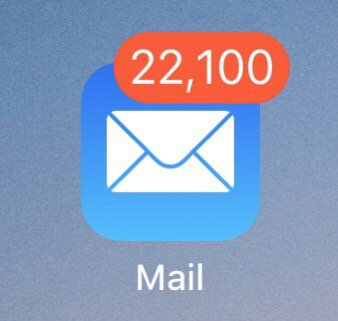
\includegraphics[width=.99\textwidth]{figures/email.jpeg}
        
        \column{.20\textwidth} % Right column and width
        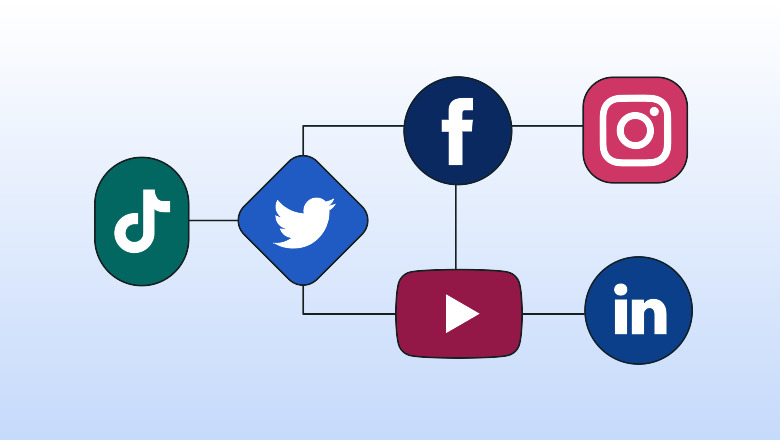
\includegraphics[width=.99\textwidth]{figures/social.jpg}

        \column{.10\textwidth} % Right column and width
        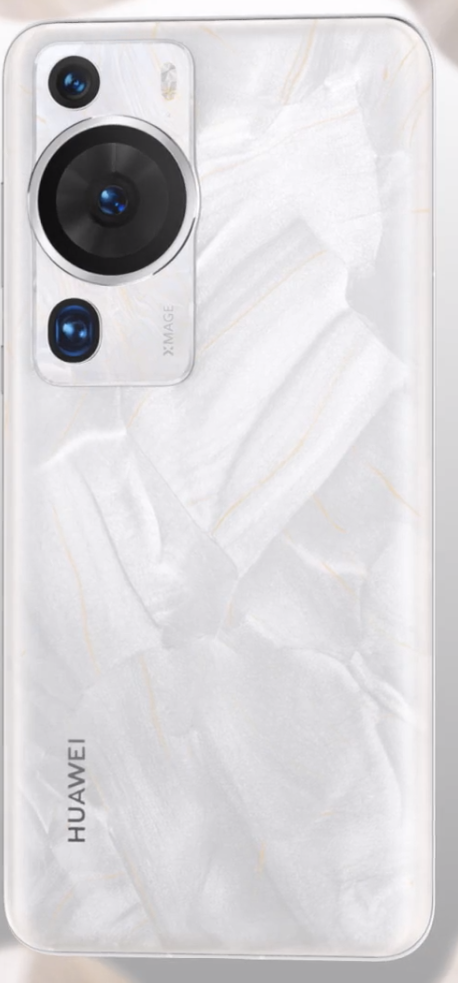
\includegraphics[width=.8\textwidth]{figures/mobilephone.png}
    \end{columns}

    Each image pixels are data, each video frames are data. 
\end{frame}

%------------------------------------------------

\begin{frame}{Collecting Data through Survey and Experiments}
    In addition, we can also collect data. An example is the US Census Bureau which collects data for making informed decisions about future policies to help businesses and citizens.

    \begin{gradblock}{}
        Running surveys is one of the prime sources of data collection in healthcare.
    \end{gradblock}
     \begin{gradblock}{}
        Field experiments to collect data: for example cars with on-board sensors as well as augmented sensors driving on streets provide information about traffic, pedestrians, etc.
    \end{gradblock}

      \begin{columns}[c] % The "c" option specifies centered vertical alignment while the "t" option is used for top vertical alignment

        \column{.35\textwidth} % Left column and width
        \includegraphics[width=.9\textwidth]{figures/patientsurvey.jpeg}

        \column{.35\textwidth} % Right column and width
        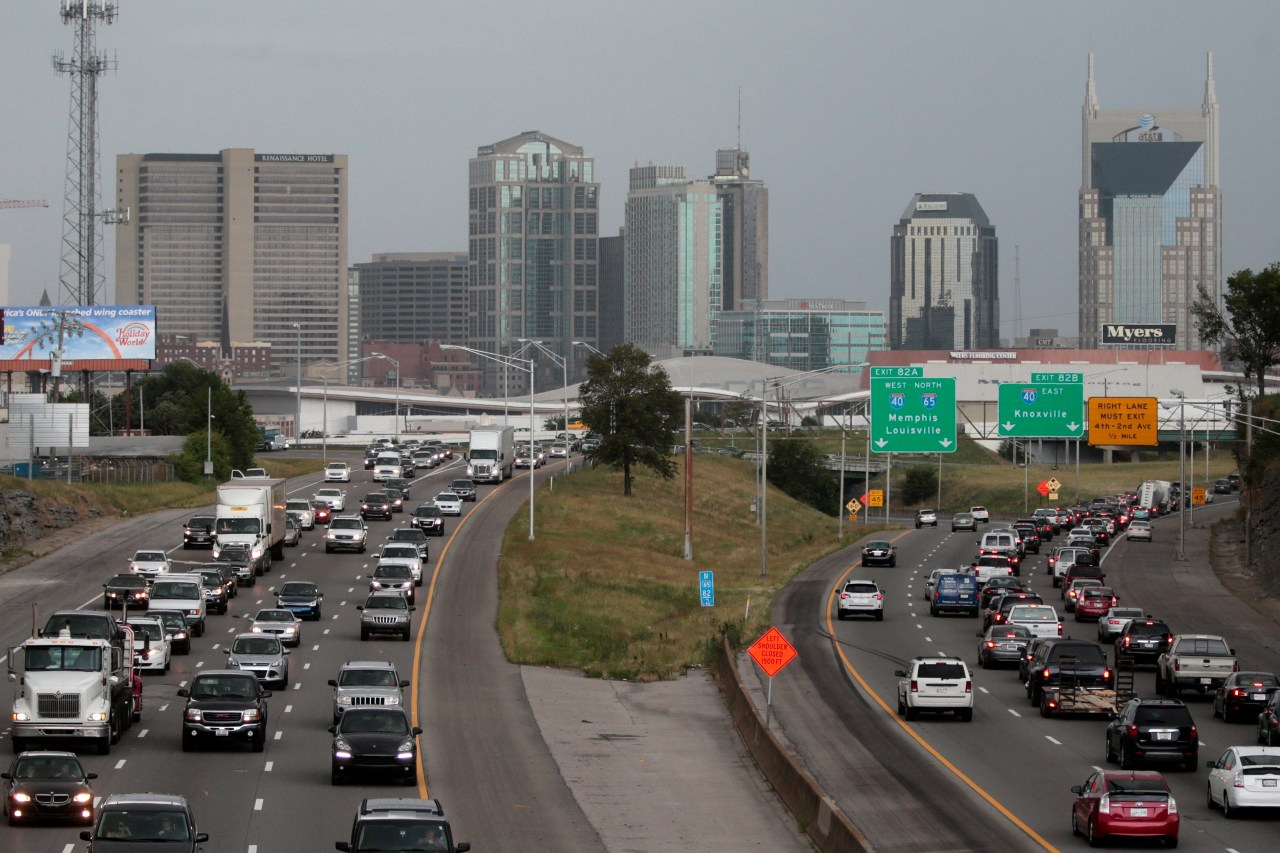
\includegraphics[width=.9\textwidth]{figures/traffic.jpeg}

    \end{columns}
    \end{frame}


% %------------------------------------------------
% \subsection{Data Collection Consideration}
% %------------------------------------------------

% %------------------------------------------------
% \begin{frame}{}
% \begin{center}
%     \Large \bf \color{DarkRed}
%     Data Collection Consideration
% \end{center}
% \end{frame}

\begin{frame}{How Data will be Collected}

    \begin{gradbox}{}
    \Large  \color{Blue}
        Consider an example question: ``What is causing increased rush hour traffic in your city?"
    \end{gradbox}

    \begin{gradblock}{\quad}
        The first step we can think of is to validate whether we get traffic congestion during rush hour. We observe the traffic pattern by counting the number of cars on city streets during particular times. 
        \\\hspace*{\fill} Data may tell us that cars are being backed up on specific streets.
    \end{gradblock}
\end{frame}

%------------------------------------------------
\begin{frame}[allowframebreaks]{Data Sources}

\begin{gradblock}{First party}
    This is the data you collect through experiments and surveys. Consider this to be the most reliable as you know how you are collecting this data.
\end{gradblock}

\begin{gradbox}{Second party}
    Second-party data is collected by a group directly from its audience and then sold. For example, if you are unable to collect your data because conducting a new experiment is hard, time-consuming, and logistically challenging, you might be able to buy it from an organization or a group that has already led the traffic pattern study in your city.

    The data is still reliable as it comes from a source that has some experience in traffic analysis.

    You may get traffic data from a research lab that recently concluded a traffic experiment. 

    Example: {\color{red}\url{https://i24motion.org/}}

    You can request an account at {\color{red}\url{https://i24motion.org/}} to download relevant datasets.
\end{gradbox}

\begin{facts}{Third party}
This type of data is collected from outside sources who did not collect it directly or they didn't collect it for the purpose you are going to use the data.

\begin{itemize}
    \item Third-party data comes from a number of different sources.
    \item Data needs to be investigated further for accuracy, bias, credibility, and trustworthiness before it can be used as it is not as reliable as second or first-party data.
    \item Example of traffic data: from HERE Map API, Google Map API; and other data aggregator services. Data sold by various companies who have aggregated user data from various social media, by the fine prints of T\&C of online contracts, etc.
\end{itemize}
    
\end{facts}
\end{frame}

%------------------------------------------------
\begin{frame}[c]{How much data to collect?}
When you’re gathering your own data, it’s crucial to make sensible choices about the sample size. For some projects, a random selection from existing data may suffice. However, other projects may require a more targeted approach to data collection, concentrating on specific criteria. Remember, each project has unique requirements.
\end{frame}

%------------------------------------------------

\begin{frame}[c]{Population}
\begin{gradblock}{Definition}
    All possible values in a certain dataset.
   \textbf{Example: If analyzing data about car traffic in a city, your population is all cars in the area.}
\end{gradblock}
\end{frame}

%------------------------------------------------


\begin{frame}[c]{How much data to collect?}
\Large
\begin{center}
    However, collecting data from the entire population can be challenging, and may not be feasible at all.
\end{center}

\end{frame}

%------------------------------------------------

\begin{frame}[c]{Sample}


\begin{gradblock}{Definition}
    A part of a population that is a representative of the population.

   \textbf{Example: You might collect data about traffic from one spot in the city and analyze or you might pull random samples from all existing data in the population.}
\end{gradblock}

\end{frame}

%------------------------------------------------
\begin{frame}{Data Formats}
    \begin{enumerate}
        \item \textbf{Quantitative Data:} Can be measured, counted, and expressed as numbers.
        \begin{enumerate}
            \item Discrete
            \item Continuous
        \end{enumerate}
        \item \textbf{Qualitative Data:} Name, category, description -- cannot be measured or counted
        \begin{enumerate}
            \item Nominal: can be categorized without a set order. Example: \{yes, no, not sure\}
            \item Ordinal: set order is important. Example: movie ratings 1-5 stars.
        \end{enumerate}
    \end{enumerate}
\end{frame}

%------------------------------------------------

\begin{frame}{Data Format Hands On}
We will use some example datasets from \textbf{A Large-Scale Sequential Dataset for Vehicle-Infrastructure (V2X) Cooperative Perception and Forecasting}: {\color{red}\url{https://github.com/AIR-THU/DAIR-V2X-Seq/}}.
\vskip 2em
Download my local copy of the example dataset from {\color{red}\url{https://drive.google.com/file/d/13jvC5YhMpdqlXyrK-IJJuEoZBmAlNzOz/view?usp=sharing}}.

\end{frame}

%------------------------------------------------
{
\usebackgroundtemplate{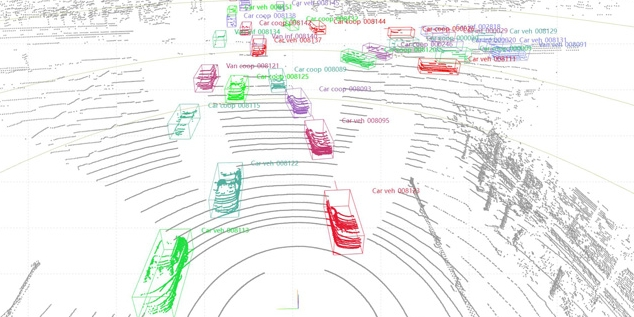
\includegraphics[width=\paperwidth]{figures/tracking.664c0f13.jpg}}%
\begin{frame}{About the V2X Dataset}
\Large
   \textbf{ V2X-Seq is a large-scale, real-world, and sequential V2X dataset, which includes data frames, trajectories, vector maps, and traffic lights captured from natural scenery.}
\end{frame}
}

%------------------------------------------------
\begin{frame}[containsverbatim, allowframebreaks]{Reading the Data from Python}
We will be reading the Trajectory forecasting dataset with an infrastructure view using the Panda package from Python.

\begin{minted}
[
framesep=1mm,
baselinestretch=1.2,
fontsize=\normalsize,
bgcolor=Apricot,
]
{python}
import pandas as pd
datadir = '../cooperative-trajectories/train/data/'
datafile = '1002.csv'

df = pd.read_csv(datadir + datafile)
df.head() # to display a portion of data 
\end{minted}
\newpage
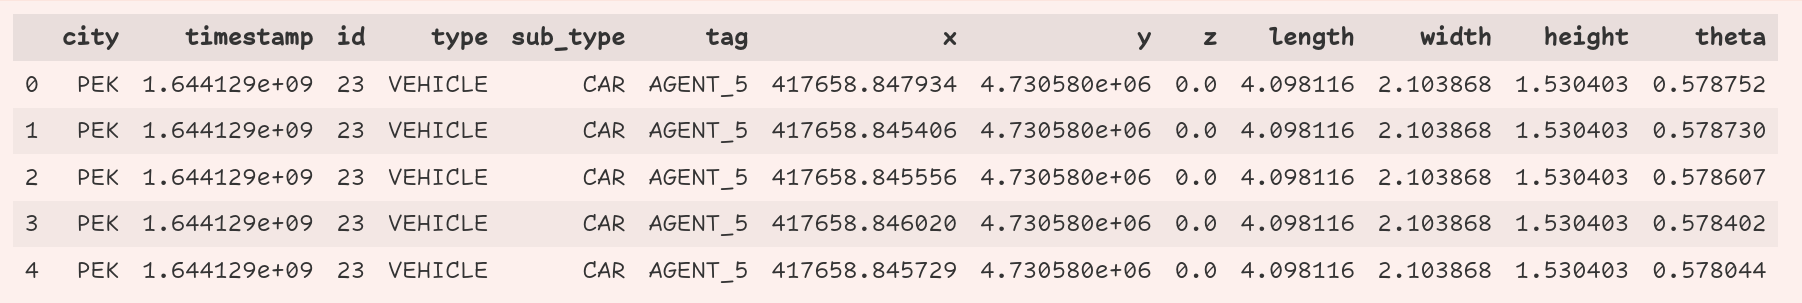
\includegraphics[width=\textwidth]{figures/V2Xtrajectory_panda_head.png}

\begin{center}
{\Large \color{red} \textbf{Which of the above columns are quantitative data, and which of them are qualitative data?}}
\end{center}
\end{frame}
%------------------------------------------------
\begin{frame}{Structured and Unstructured Data}

\begin{enumerate}
    \item \textbf{Structured Data:} Data organized in a certain format such as rows and columns.
    \begin{itemize}
        \item[-] Spreadsheets
        \item[-] Relational databases
        \item[-] JSON format datasets
    \end{itemize}

{\color{Purple}Structured data works nicely within a data model, which is a model that is used for organizing data elements and how they are related to one another.}
\begin{gradblock}{Data elements}
    A piece of information such as student's name, A\# number, residential address, etc.
\end{gradblock}
    \item \textbf{Unstructured Data:}
        \begin{itemize}
            \item[-] Audio
            \item[-] Video
            \item[-] Emails
            \item[-] Photos
        \end{itemize}
\end{enumerate}
\end{frame}

%------------------------------------------------
\begin{frame}{Data Model}
    \begin{facts}{}
        \begin{itemize}
            \item The Data model helps to keep data consistent and provides a map of how data is organized.
            \item Having a data model makes it easier for data engineers and analysts to communicate about data to other stakeholders to make sense of their data and use it to make business decisions.
            \item Helpful in creating visualization tool.
        \end{itemize}
    \end{facts}

    An example of a data model can be seen in: {\color{red}\url{https://github.com/AIR-THU/DAIR-V2X-Seq/blob/main/dataset/v2x-seq-tfd/README.md}}.
\end{frame}
%------------------------------------------------
\begin{frame}{Metadata}
    \begin{facts}{Definition}
        An abstract concept used to describe your data.
        \textbf{Example:} Smartphone picture taken from your phone has metadata such as image size, ISO, geolocation tagged, timestamp of the image acquisition, etc.
    \end{facts}
\end{frame}

%------------------------------------------------
\section{Data Visualization}
%------------------------------------------------

%------------------------------------------------
\begin{frame}{}
\begin{center}
    \huge \bf \color{DarkRed}
    Data Visualization
\end{center}
\end{frame}

%------------------------------------------------

\begin{frame}{Why Data Visualization?}

\Large 
\begin{center}
     Being able to present data and insights in a clear, engaging, and accessible manner is a key competency for successful data scientists and analysts. This skill transforms data into a captivating narrative.
\end{center}
   
\end{frame}

%------------------------------------------------

\begin{frame}{Why Data Visualization?}

\Large 
\begin{center}
    \begin{enumerate}
        \item Highlights and reveals patterns, trends, and relationships.
        \item Simplifies the data for stakeholders.
        \item Presents data for better understanding and interpretation
    \end{enumerate}
\end{center}
   
\end{frame}


%------------------------------------------------

\begin{frame}{Power of Data Visualization}
    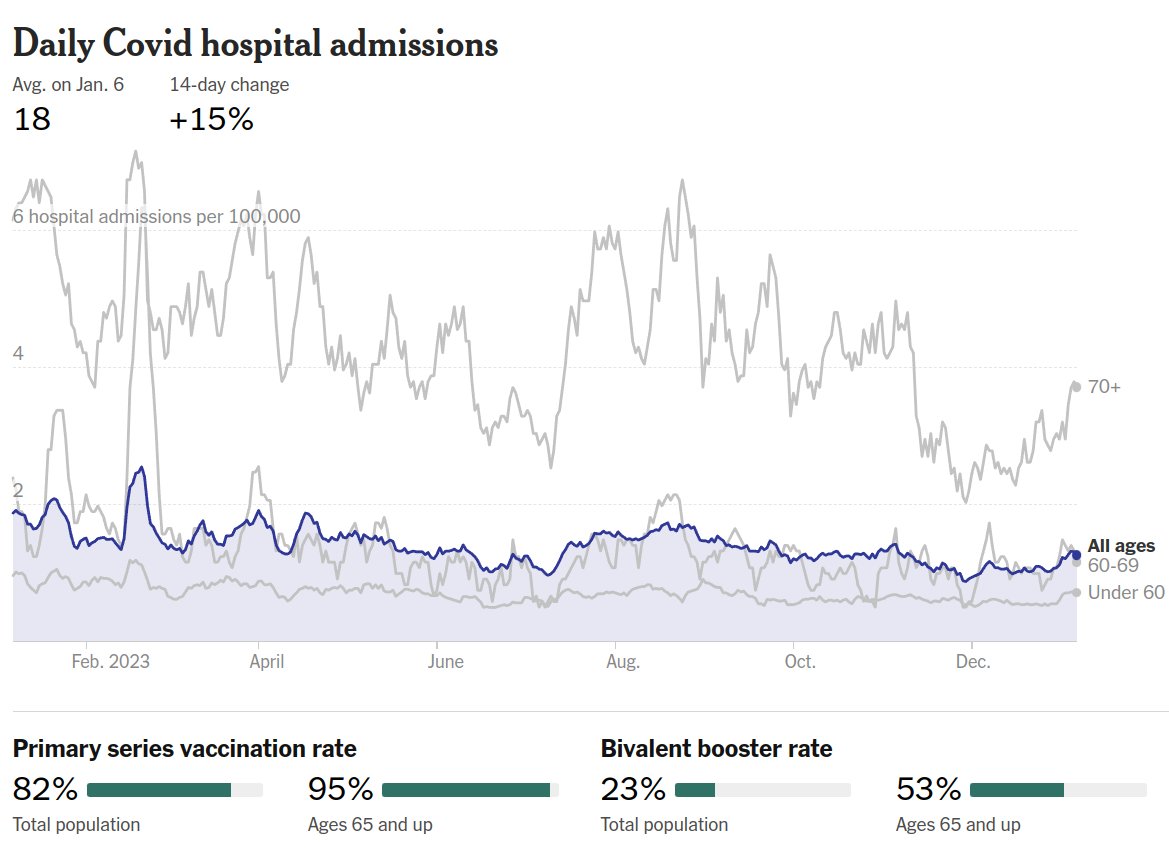
\includegraphics[width=0.49\textwidth]{figures/covid19hawaii.png}
    
    {\textbf{Source: }\color{red} \url{https://www.nytimes.com/interactive/2023/us/hawaii-covid-cases.html}}
\end{frame}


%------------------------------------------------
\begin{frame}{Data Visualization Best Practices}
\begin{enumerate}
    \item Choosing the right type of visualization.
    \begin{itemize}
        \item[-] Different types of data require different visualization techniques
    \end{itemize}
    \item Keep it simple
    \begin{itemize}
        \item[-] Line chart for trends and bar chart for comparison
    \end{itemize}
    \item Label axes properly, use clear formatting
    \begin{itemize}
        \item[-] Use a suitable title and legend
    \end{itemize}
    \item Less is more.
\end{enumerate}
\end{frame}


\begin{frame}{Example}

{\color{purple}\url{https://miro.medium.com/v2/resize:fit:640/format:webp/1*ZF-3-ih4QwSVTVXZeVV-iA.gif}}
\end{frame}
%------------------------------------------------

\begin{frame}{Broader Types of Data Visualization}
\Large
\begin{enumerate}
    \item Graphical representation of data and information
    \item Basic charts and graphs
    \item Interactive dashboards and maps
\end{enumerate}
    
\end{frame}

%------------------------------------------------
\begin{frame}{Most Basic Types of Plots}
    \begin{enumerate}
        \item Line Plot
        \item Bar Plot
        \item Scatter Plot
        \item Histogram
        \item KDE Plot
        \item Box Plot
    \end{enumerate}
\end{frame}

%------------------------------------------------
\begin{frame}[allowframebreaks, containsverbatim]{Line Plot}
\begin{columns}[c]
    \column{.40\textwidth}
    \begin{enumerate}
        \item Displays trend over time
        \item Connects two subsequent points in the dataset using a straight line
        \item The visual of the line plot depends on the order of data points.
        \item Illustrate cause-effect relationship.
    \end{enumerate}
    \column{.60\textwidth}
    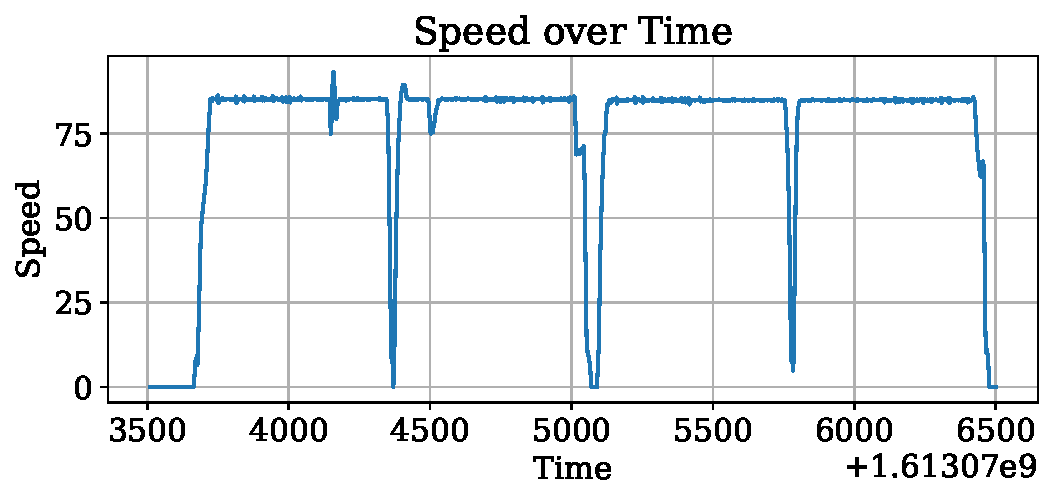
\includegraphics[width=0.99\textwidth]{figures/lineplot.pdf}
    \end{columns}
\vskip 2em
    Download a Toyota RAV4 driving dataset from {\color{red}\url{https://drive.google.com/file/d/1UPRgg9HFNlcvud31kTfOI7Zc59x0J8Z_/view?usp=sharing}}
\begin{minted}
[
framesep=1mm,
baselinestretch=1.2,
fontsize=\normalsize,
bgcolor=Thistle,
]
{python}
data_df = pd.read_csv(datadir + datafile, index_col=0)
data_df.head()
# Create the plot
plt.figure(figsize=(8, 3))  # Increase the size of the plot
plt.plot(data_df['Time'], data_df['speed'])
# Add labels and title
plt.xlabel('Time')
plt.ylabel('Speed')
plt.title('Speed over Time')
# Show grid
plt.grid(True)
\end{minted}
\end{frame}

%------------------------------------------------
\begin{frame}[allowframebreaks, containsverbatim]{Bar Plot}
\begin{columns}[c]
    \column{.40\textwidth}
    \begin{enumerate}
        \item Displays data using rectangular bars
        \item Height of data represents the magnitude of data
        \item Helpful in displaying data that has different categories
        \item Compare different categories and groups
        \item Can also visualize data that can be ranked or ordered
    \end{enumerate}
    \column{.60\textwidth}
    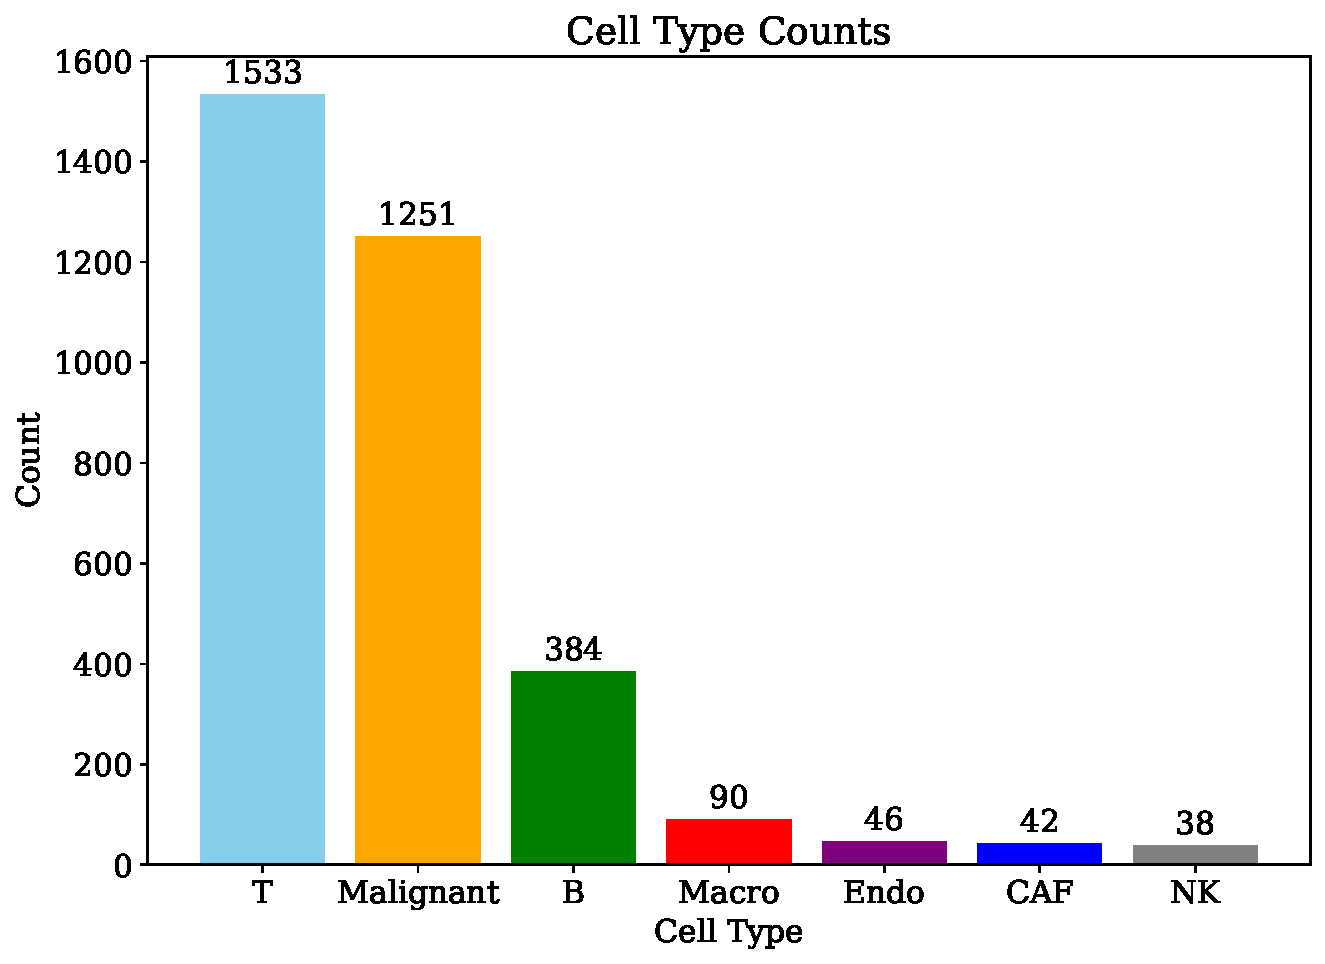
\includegraphics[width=0.99\textwidth]{figures/barplot.pdf}
    \end{columns}
    \vskip 2em
    Download a single-cell sequencing melanoma dataset from {\color{red}\url{https://drive.google.com/drive/folders/1XepEHBAkpdi7_uUy3cUC12G1ckACw3Dv?usp=sharing}}. They contain single-cell samples, with genes as features and each entries are gene-expression levels.

\vskip 2em
Original data source: \url{https://www.ncbi.nlm.nih.gov/geo/query/acc.cgi?acc=GSE72056}.
    
\vskip 2em
{
    \textbf{Reference:}
    \footnotesize{
        \begin{thebibliography}{99}
            \bibitem[Bioconductor, 2007]{p1} Introduction to Single-Cell Analysis with Bioconductor, {\color{purple}\url{https://bioconductor.org/books/3.14/OSCA.intro/getting-scrna-seq-datasets.html}}
        \end{thebibliography}
    }
}
\vskip 2em
We will visualize how many of each of the cell types are present using a bar plot.

\begin{minted}
[
framesep=1mm,
baselinestretch=1.2,
fontsize=\footnotesize,
bgcolor=Thistle,
]
{python}
counts = data_df['type'].value_counts()
plt.figure(figsize=(10,7))
# Set the global font to be Serif, size 15
plt.rcParams['font.family'] = 'Serif'
plt.rcParams['font.size'] = 15
# Define a color list
colors = ['skyblue', 'orange', 'green', 'red', 'purple', 'blue', 'gray']
bars = plt.bar(counts.index, counts.values, color=colors)
# Adding counts on the top of each bar
for bar in bars:
    yval = bar.get_height()
    plt.text(bar.get_x()+bar.get_width()/2, yval+10, yval, ha='center', va='bottom')
plt.xlabel('Cell Type')
plt.ylabel('Count')
plt.title('Cell Type Counts')
\end{minted}
\end{frame}
    
%------------------------------------------------
\begin{frame}[allowframebreaks, containsverbatim]{Scatter Plot}
\begin{columns}[c]
    \column{.40\textwidth}
    \begin{enumerate}
        \item Good to visualize one variable against another variable
        \item The ordering of data doesn't affect the visualization
        \item Helpful in detecting outliers and unusual observations
        \item Compare different categories and groups
        \item Identify clusters or groups in the data
    \end{enumerate}
    \column{.60\textwidth}
    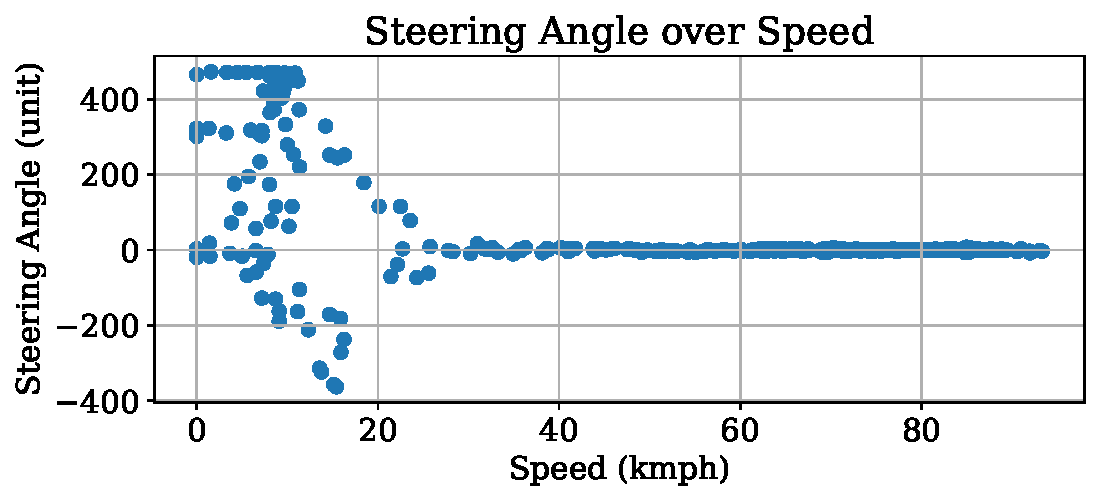
\includegraphics[width=0.99\textwidth]{figures/scatterplot.pdf}
    \end{columns}

\vskip 2em
We will visualize how the steering angle is related to speed in the case of the RAV4 driving dataset.



\begin{minted}
[
framesep=1mm,
baselinestretch=1.2,
fontsize=\footnotesize,
bgcolor=Thistle,
]
{python}
plt.scatter(data_df['speed'], data_df['steer_angle'])

# Add labels and title
plt.xlabel('Speed')
plt.ylabel('Steering Angle')
plt.title('Steering Angle over Speed')
\end{minted}

\end{frame}


%------------------------------------------------
\begin{frame}[allowframebreaks, containsverbatim]{Histogram}
A special type of bar graph that displays variations in data like time, speed, weight, etc. A histogram enables a team to recognize and analyze patterns in data that are not apparent simply by looking at a
table of data, or by finding the average or median.
   \begin{gradbox}{}
       Histograms are approximations of data distribution.
   \end{gradbox}

Histograms are constructed by dividing $n$ measurements of a sample into $b$ bins or classes (also called intervals). In such a case, we have the first bin $b = 1$ representing a data range for $x_1 < x < x_2$, the second bin $b= 2$, $x_2 < x < x_3$, and so on.

\vskip 2em 
The middle point of each bin $j$ is $x_{mid,j} = \tfrac{x_j + x_{j+1}}{2}$. The number of observations within each bin $j$, called frequency is plotted as a bar graph for each bin.

    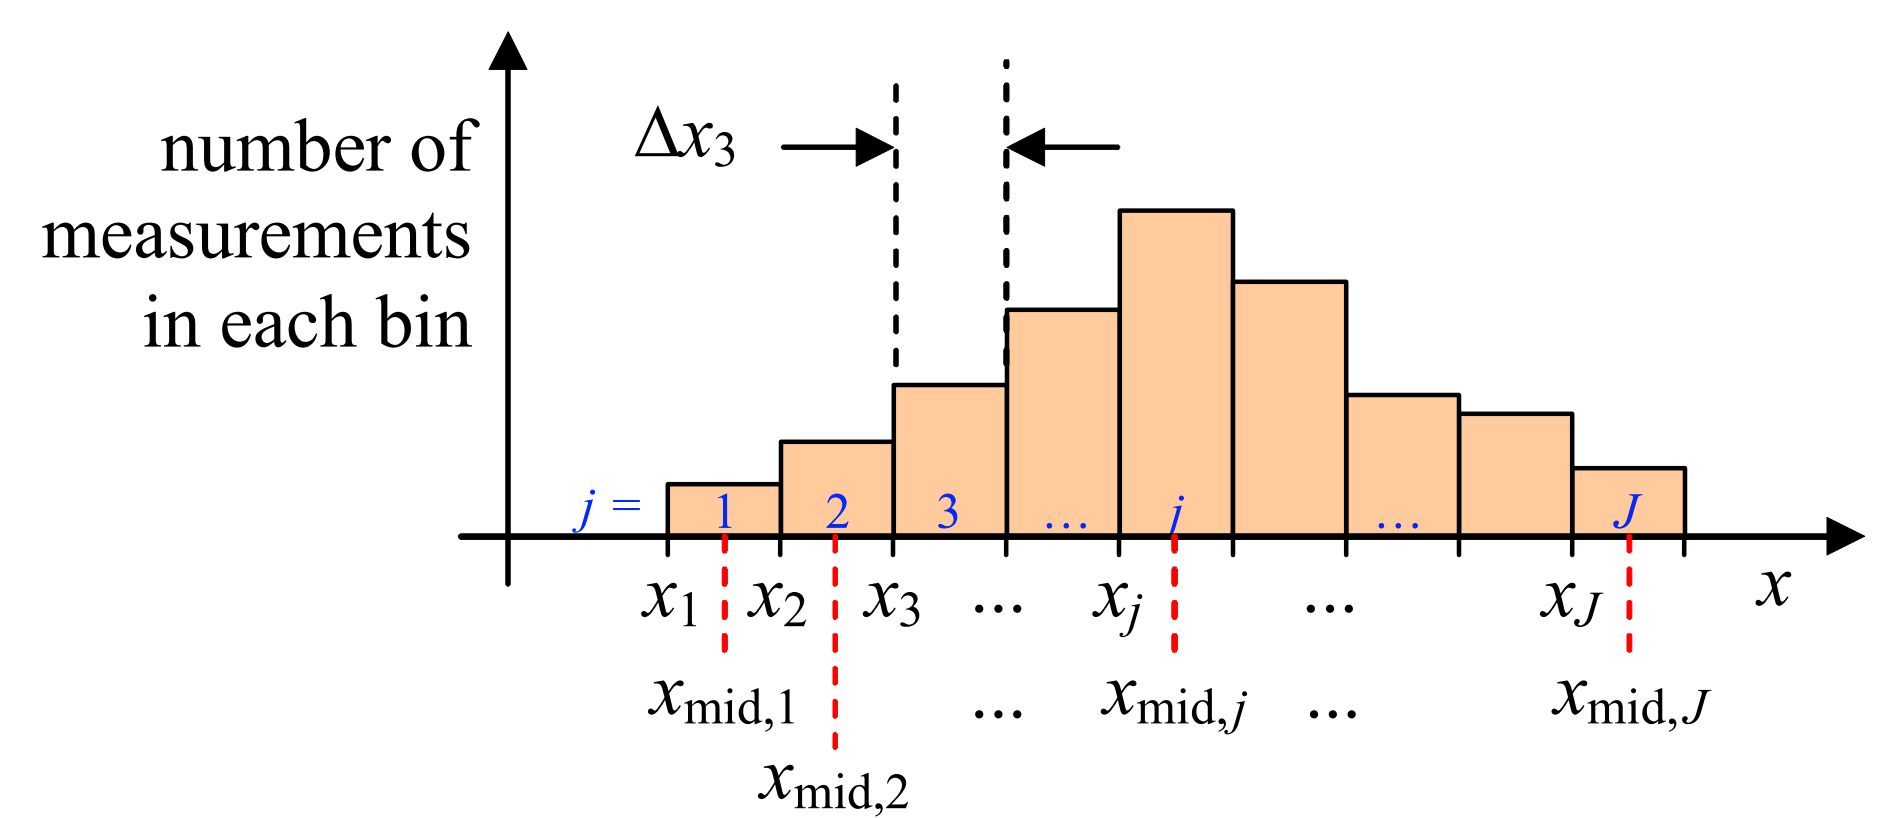
\includegraphics[width=0.89\textwidth]{figures/histogram_bins.png}
\begin{gradbox}{How to choose the number of bins?}
    \begin{enumerate}
        \item Sturgis rule: $B = 1 + 3.3\log_{10} n$
        \item Rice rule: $B = 2 n^{\tfrac{1}{3}}$
    \end{enumerate}
\end{gradbox}

\begin{facts}{Probability Histogram}
    If you divide the vertical axis (the frequency axis) by the total number of measurements, the resulting histogram is called \textbf{probability histogram}. We can also define 
    \begin{equation}
        \text{probability}_b = \cfrac{\text{the number of measurements in the bin j}}{n}
    \end{equation}
\end{facts}
\begin{gradbox}{Vertically Normalized Histogram}
    A histogram obtained by further dividing the
vertical axis by the bin width is called a vertically normalized histogram.
interval width. The vertical axis of the
the vertically normalized histogram is defined as
\begin{equation}
    f(x_{mid,j} ) =  \cfrac{\text{the number of measurements in the bin j}}{\Delta x_j \cdot n}
\end{equation}
 This makes sure that mathematically the area of the bin is equal to the probability that $x$ lies in that bin. 
\end{gradbox}

    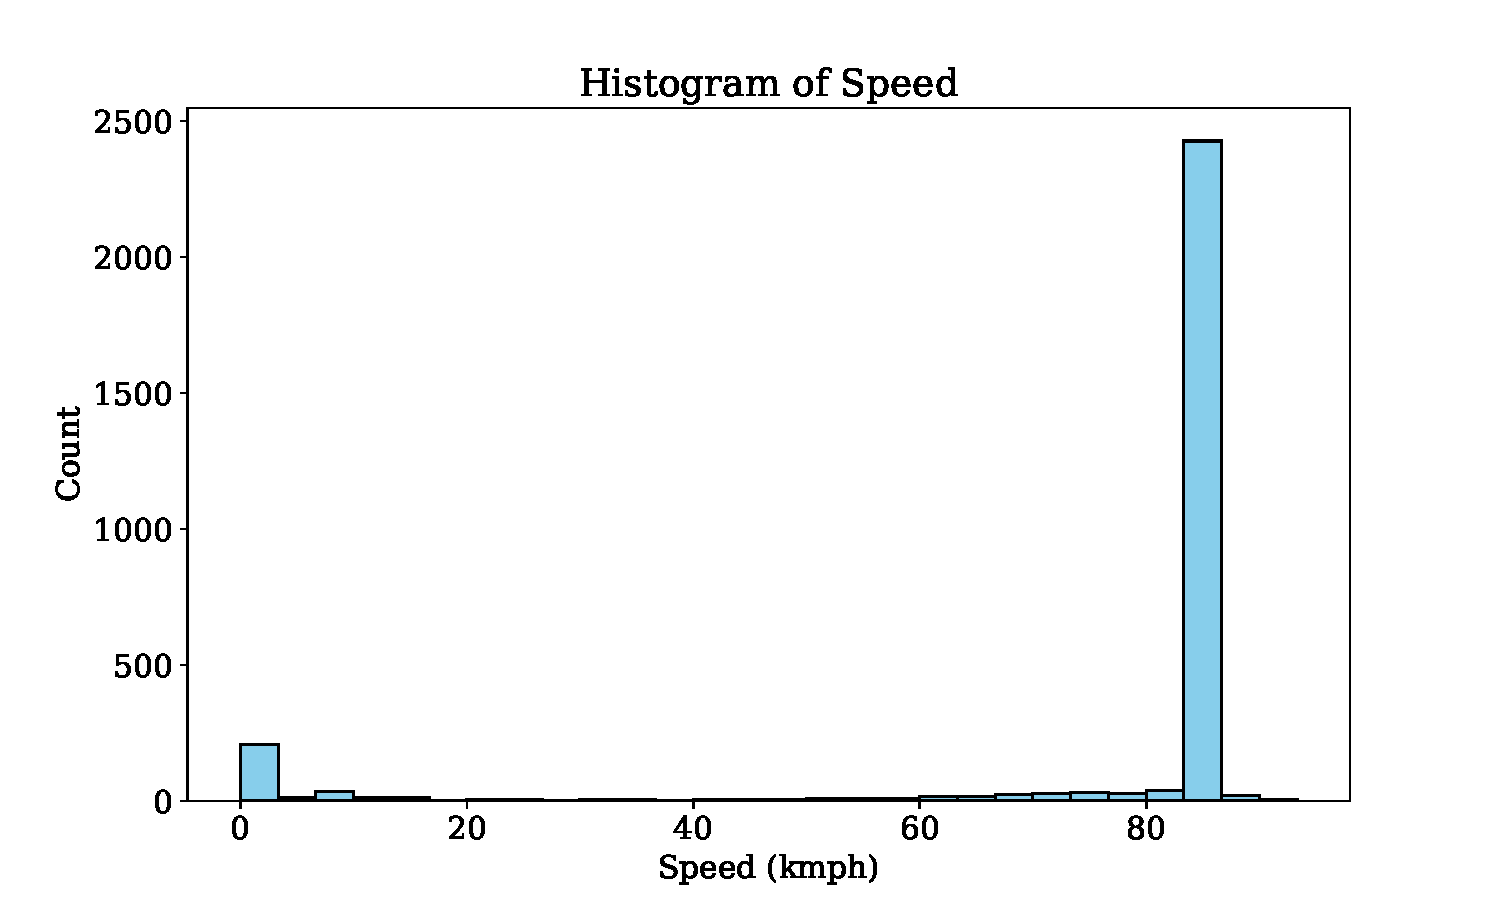
\includegraphics[width=0.79\textwidth]{figures/histogram.pdf}


\end{frame}
%=======================================================
\begin{frame}[containsverbatim]{Histogram Plot}
\begin{minted}
[
framesep=1mm,
baselinestretch=1.2,
fontsize=\footnotesize,
bgcolor=Thistle,
]
{python}
n = len(data)
num_bins = int(2 * n**(1/3))
plt.figure(figsize=(10,6))
plt.hist(data, bins=num_bins, color='skyblue', edgecolor='black')
plt.xlabel('Speed (kmph)')
plt.ylabel('Count')
plt.title('Histogram of Speed')
\end{minted}
\end{frame}


%================================================
\begin{frame}[containsverbatim]{Vertically Normalized Histogram Plot}
Set \texttt{density=True} to create vertically normalized histogram
\begin{columns}[c]
    \column{.50\textwidth}
\begin{minted}
[
framesep=1mm,
baselinestretch=1.2,
fontsize=\footnotesize,
bgcolor=Violet,
]
{python}
n = len(data)
num_bins = int(2 * n**(1/3))
plt.figure(figsize=(10,6))
plt.hist(data, bins=num_bins, 
    density=True, color='skyblue', 
    edgecolor='black')
plt.xlabel('Speed (kmph)')
plt.ylabel('Probability')
plt.title('Histogram of Speed')
\end{minted}
\column{.50\textwidth}
    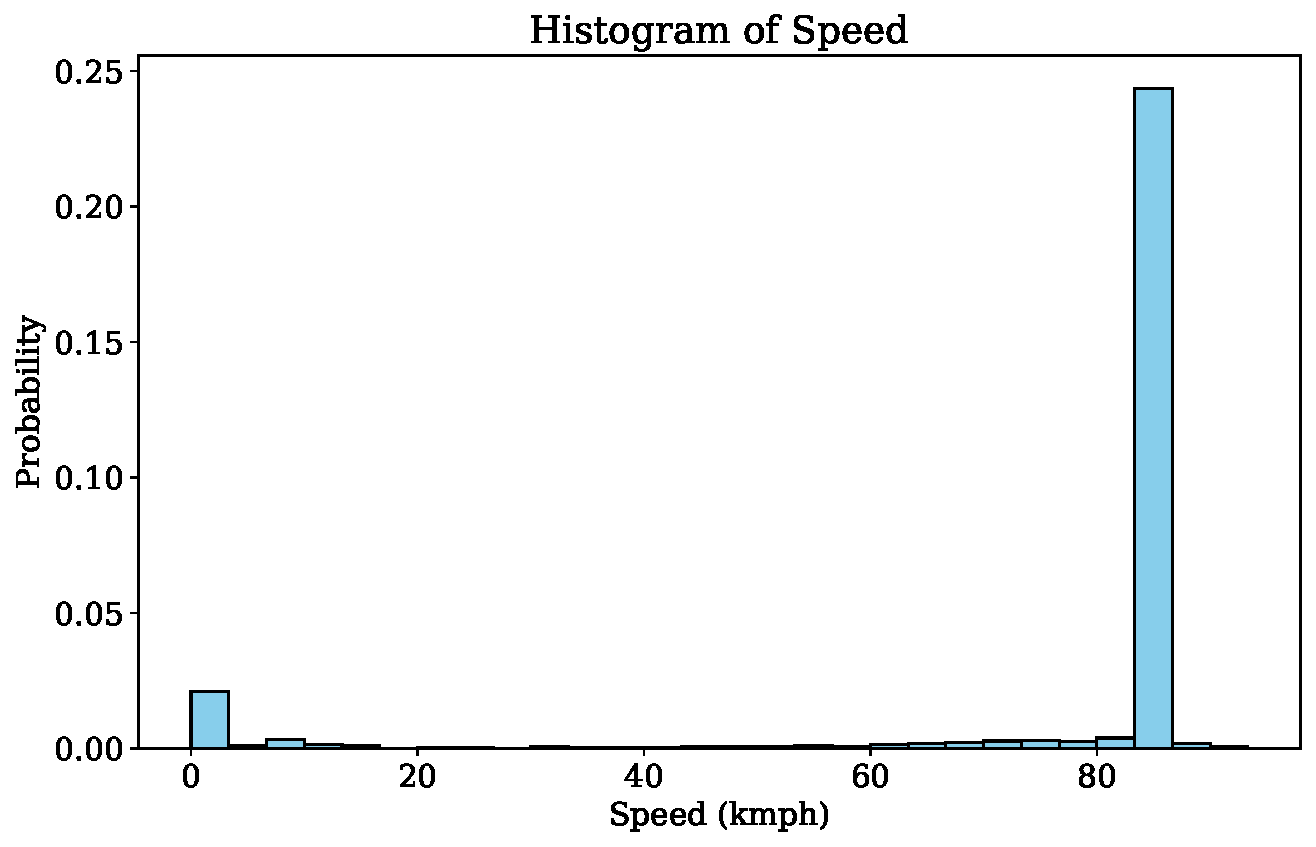
\includegraphics[width=1.09\textwidth]{figures/histogram_normal.pdf}

\end{columns}

\vskip 1em
{
    \textbf{Further Reading:}
    \footnotesize{
        \begin{thebibliography}{99}
            \bibitem[Histogram]{p2} Histogram, {\color{purple}\url{https://www.me.psu.edu/cimbala/me345/Lectures/Histograms.pdf}}
        \end{thebibliography}
    }
}


\end{frame}
%------------------------------------------------

\begin{frame}[allowframebreaks]{Kernel Density Estimation Plot}
\begin{facts}{Kernel Density Estimation (KDE)}
Kernel density estimation's goal is to estimate the probability density function from a given dataset. The KDE is given by 
\begin{equation}
    \phat_n(x) = \cfrac{1}{nh}\sum_{i=1}^n K\bigg( \cfrac{X_i - x} {h}\bigg)
\end{equation}
    where $K(x)$ is called \textbf{kernel function} which is generally smooth and symmetric. $h$ is called smoothing bandwidth which controls the amount of smoothing. $X_i$ is a data point. $n$ is the total number of data points. KDE smoothes each data point into a small density bumps and them sum all these bumps together to obtain the final density estimate.
\end{facts}

\begin{gradblock}{Smoothing Bandwidth in KDE}
    If we have a smaller bandwidth $h$, it will result in under smoothing, more wiggly curve. If $h$ is too large, it will cause over-smoothing and some important structures might not be revealed.
\end{gradblock}

    
\begin{gradbox}{Kernel Function}
     A kernel function should have following properties:
     \begin{enumerate}
         \item $K(x)$ must be symmetric.
         \item $\int K(x)dx = 1$.
         \item $\lim_{x\to-\infty} K(x) = \lim_{x\to+\infty} K(x) = 0$.
     \end{enumerate}
\end{gradbox} 

\begin{facts}{Some Common Kernel Functions}
\begin{enumerate}
    \item Gaussian: $K(x)= \cfrac{1}{\sqrt{2\pi} e^{-x^2/2}}$.
    \item Uniform: $K(x) = \cfrac{1}{2}I(-1 \leq x \leq 1)$, \quad $I$ is an identity function.
    \item Epanechnikov: $K(x) = \cfrac{3}{4}\cdot \max(1 - x^2, 0)$.
\end{enumerate}
\end{facts}
\end{frame}

%------------------------------------------------

\begin{frame}[allowframebreaks, containsverbatim]{Kernel Density Estimation Plot with Python}
\begin{columns}[c]
    \column{.50\textwidth}
\begin{minted}
[
framesep=1mm,
baselinestretch=1.2,
fontsize=\footnotesize,
bgcolor=Moccasin,
]
{python}
n = len(data)
num_bins = int(2 * n**(1/3))
plt.figure(figsize=(10,6))
# Plot histogram
plt.hist(data, bins=num_bins, density=True,
    color='skyblue', edgecolor='black', 
    alpha=0.5)
# Overlay KDE plot
sns.kdeplot(data, color='darkblue', 
    bw_adjust=1.0)
plt.xlabel('Speed (kmph)')
plt.ylabel('Density')
plt.title('Histogram/KDE Plot of Speed')
\end{minted}
\column{.50\textwidth}
    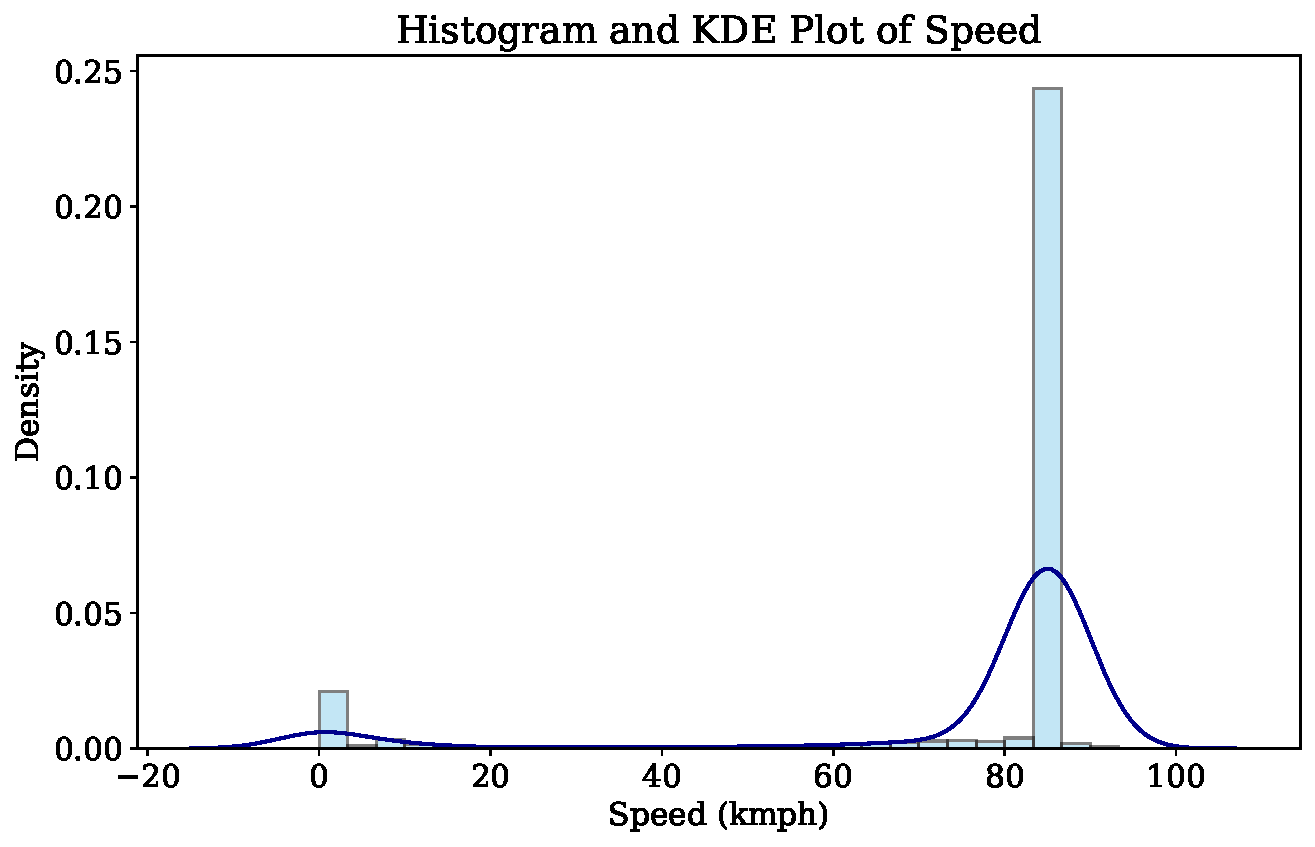
\includegraphics[width=1.09\textwidth]{figures/histogram_kdeplot.pdf}
\end{columns}

\vskip 1em
{
    \textbf{Further Reading:}
    \footnotesize{
        \begin{thebibliography}{99}
            \bibitem[KDEPLOT]{p3} Fast \& Accurate Gaussian Kernel Density Estimation, {\color{purple}\url{https://web.archive.org/web/20240124222356/https://idl.cs.washington.edu/files/2021-FastKDE-VIS.pdf}}
        \end{thebibliography}
    }
}
\end{frame}

%------------------------------------------------

\begin{frame}[allowframebreaks, containsverbatim]{Boxplot}
\begin{columns}[c]
    \column{.50\textwidth}
\begin{enumerate}
    \item Summarizes data into a `5-number' summary.
    \item Detects extreme observation
    \item The Centerline marks the median.
    \item Box plots characterize a sample using the 25th, 50th, and 75th
percentiles—also known as the lower quartile (Q1), median (m or
Q2) and upper quartile (Q3)—and the interquartile range (IQR =
Q3 – Q1), which covers the central 50\% of the data.
\end{enumerate}
 \column{.50\textwidth}
 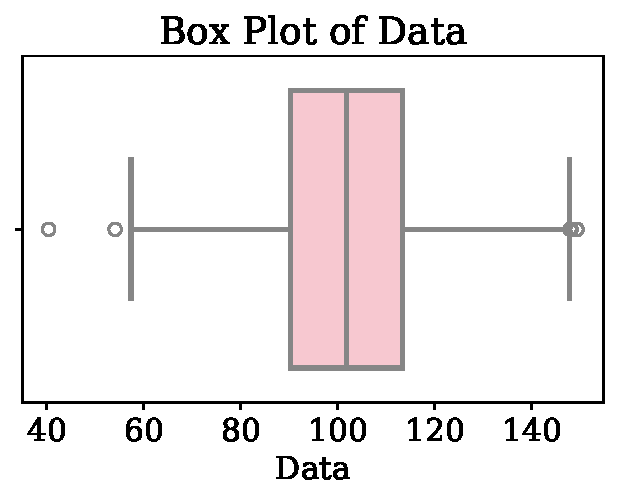
\includegraphics[width=1.09\textwidth]{figures/boxplot.pdf}
\end{columns}
\end{frame}


%------------------------------------------------

\begin{frame}[allowframebreaks, containsverbatim]{But Why Quartiles?}
\begin{columns}[c]
    \column{.50\textwidth}
\begin{enumerate}
    \item Quartiles are
insensitive to outliers and preserve information about the center and
spread. 
\item  They are preferred over the mean and variance for
population distributions that are asymmetric or irregularly shaped
and for samples with extreme outliers.
\item There is a special plot called \textbf{violin plot} that combines boxplot with kernel density estimation.
\end{enumerate}
 \column{.50\textwidth}
 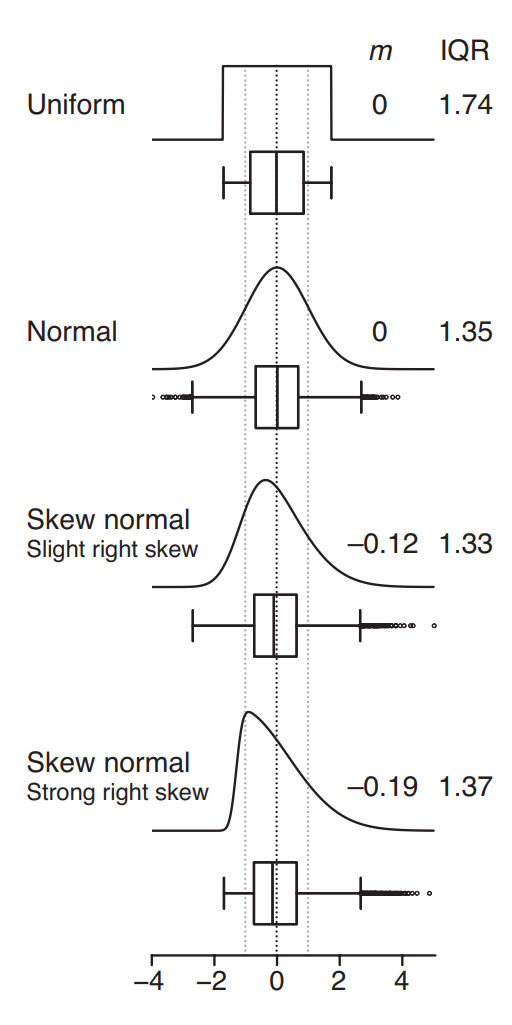
\includegraphics[height=0.79\paperheight]{figures/boxplot_distributions.png}
\end{columns}

\vskip 1em
{
    \textbf{Further Reading:}
    \footnotesize{
        \begin{thebibliography}{99}
            \bibitem[BOXPLOT]{p4} Visualizing samples with box plots, {\color{purple}\url{https://web.archive.org/web/20240125000715/https://course.khoury.northeastern.edu/cs7280sp16/CS7280-Spring16_files/NatureMethods-boxplots.pdf}}
        \end{thebibliography}
    }
}

\end{frame}
%------------------------------------------------
\begin{frame}[allowframebreaks, containsverbatim]{Plotting Libraries in Python}
\begin{enumerate}
    \item Matplotlib
    \item Seaborn: built on the top of Matplotlib, but comes with various color schemes and styles
    \item Panda comes with its own functions that directly let you use Matplotlib
    \item Plotly: interactive plots and dashboards; enables plotting in a web browser
    \item plotly-resampler package lets use plotly for large datasets $> 1 million$ datapoints
    \item Some other dashboarding tools: Boken, Voila, Bowtie
    
\end{enumerate}

\end{frame}



    \begin{frame}
        \Huge{\centerline{\color{MediumBlue}\textbf{The End}}}
    \end{frame}


\end{document}